%16_binary_heap.tex
%notes for the course COMS10007 taught at the University of Bristol
%Conor Houghton conor.houghton@bristol.ac.uk

%To the extent possible under law, the author has dedicated all copyright 
%and related and neighboring rights to these notes to the public domain 
%worldwide. These notes are distributed without any warranty. 

\documentclass[11pt,a4paper]{scrartcl}
\typearea{12}
\usepackage{graphicx}
\usepackage{pstricks}
\usepackage{listings}
\usepackage{tikz-qtree}
\lstset{language=C}
\usepackage{fancyhdr}
\pagestyle{fancy}
\lfoot{\texttt{github.com/conorhoughton/COMS10007}}
\cfoot{}
\rhead{\thepage}
\lhead{COMS10007 - algorithms 16\_binary\_heap - Conor}

\begin{document}
\tikzset{every tree node/.style={minimum width=2em,draw,circle},
         blank/.style={draw=none},
         edge from parent/.style=
         {draw,->, edge from parent path={(\tikzparentnode) -- (\tikzchildnode)}},
         level distance=1.5cm}

\section*{16 - binary heap}

A binary heap is a data structure which allows elements to be easily
added and removed while keeping track of the largest element. They are
important because they are used to implement priority queues in
scheduling, for example, in a router. We have actually already seen
another potential application, in Dijskra's algorithm the lowest
distance node is always evaluated next and a binary heap could be used
to track which node is the lowest. Here, for definiteness, we will
consider a tree designed to keep track of the highest node, rather
than the lowest as in the the Dijstra example, but, of course, this
isn't a significant difference.

A binary heap is a complete binary tree; a binary tree means, as ever,
that all the nodes have up to two child nodes. A complete tree is one
where all the layers except the lowest layer are full. A binary heap
also has the \textsl{heap} property which states that every node is
smaller than, or equal to, its parent. These definitions are
illustrated in Fig.~\ref{fig:example_trees}.

Of course, in a binary heap, because of the heap property, the root
node is always the biggest element. It turns out that storing data in
a binary heap is an efficient way to keep track of the biggest element
if elements are continually being added and removed, and, in
particular if the biggest element is often removed, as it is in a
priority queue.

\begin{figure}
\begin{center}
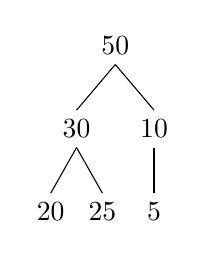
\begin{tikzpicture}
\Tree [.50 [.30 20 25 ] [.10 5 ] ];
\end{tikzpicture}
\qquad
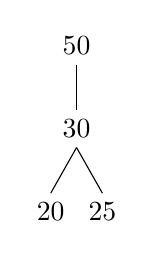
\begin{tikzpicture}
\Tree [.50 [.30 20 25 ] ];
\end{tikzpicture}
\qquad
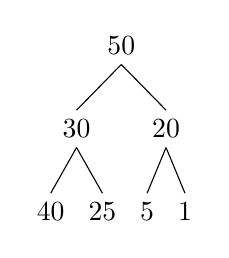
\begin{tikzpicture}
\Tree [.50 [.30 40 25 ] [.20 5 1 ] ];
\end{tikzpicture}
\end{center}
\caption{The first tree is a binary heap; it doesn't matter that the
  ten on the second row is less than elements on the third row, the
  defining propery is that nodes are bigger than their children and
  smaller than their parents. Similarly, it doesn't matter that the
  third row isn't complete, since this is the lowest row. The second
  tree isn't complete, there are gaps on the second row even though
  there are nodes on the third row. The third tree doesn't satisfy the
  heap property, the 40 is bigger than the 30 above
  it.\label{fig:example_trees}}
\end{figure}


Of course, in a binary heap, because of the heap property, the root
node is always the biggest element. It turns out that storing data in
a binary heap is an efficient way to keep track of the biggest element
if elements are continually being added and removed, and, in
particular if the biggest element is often removed, as it is in a
priority queue.

Let's first of all consider adding a new item to a binary heap. For
neatness imagine we have the rule that we fill the lowest level from
left to right. To add a new item the new node is inserted in the first
available place and then swapped upwards until the heap property is
restored. In other words, if the new node is larger than its parent it
is swapped with its parent and this it continued, with the new node
bubbling upwards, until the new node is smaller than its parent, or is
the root. This is illustrated in Fig.~\ref{fig:adding}. To create a
heap out of a list of items, add the items to the list one-by-one using this algorithm, this is sometimes called \textsl{heapifying}.

\begin{figure}
\begin{center}
$
\begin{array}{lclc}
\textbf{A}&&\textbf{B}&\\
&
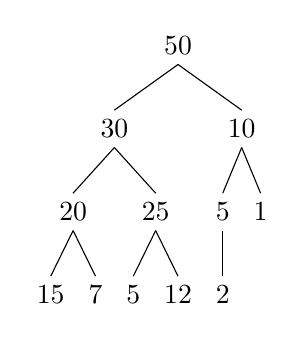
\begin{tikzpicture}
\Tree [.50 [.30 [.20 15 7 ] [.25 5 12 ] ] [.10 [.5 2 ] 1 ] ];
\end{tikzpicture}
&&
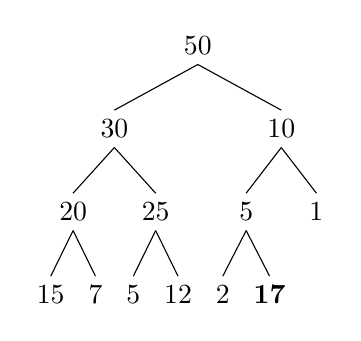
\begin{tikzpicture}
\Tree [.50 [.30 [.20 15 7 ] [.25 5 12 ] ] [.10 [.5 2 \textbf{17} ] 1 ] ];
\end{tikzpicture}
\\
\textbf{C}&&\textbf{D}&\\
&
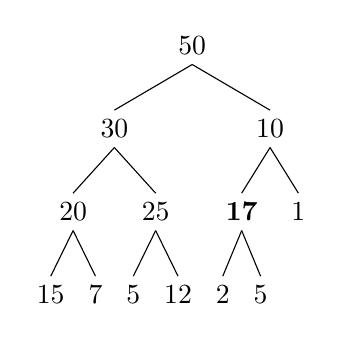
\begin{tikzpicture}
\Tree [.50 [.30 [.20 15 7 ] [.25 5 12 ] ] [.10 [.\textbf{17} 2 5 ] 1 ] ];
\end{tikzpicture}
&&
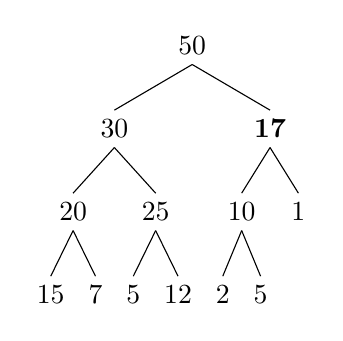
\begin{tikzpicture}
\Tree [.50 [.30 [.20 15 7 ] [.25 5 12 ] ] [.\textbf{17} [.10 2 5 ] 1 ] ];
\end{tikzpicture}
\end{array}
$
\end{center}
\caption{\textbf{A} shows the tree before the new node is added; in \textbf{B} the new node is added to the first available slot and in \textbf{C} and \textbf{D} it bubbles upwards to its correct position.\label{fig:adding}}
\end{figure}

Next lets consider removing the top node. If the top node is removed a
new node needs to be put in its place; to maintain the completeness
property this is the last node on the lowest layer, the location the
last node was added. This node is moved to the top. Now the heap
property has to be re-implimented by swapping this node down to its correct place, to do this, as long as it is smaller than either of its children it is swapped with the larger of its two children. An example is shown in Fig.~\ref{fig:removing}.

\begin{figure}
\begin{center}
$
\begin{array}{lclc}
\textbf{A}&&\textbf{B}&\\
&
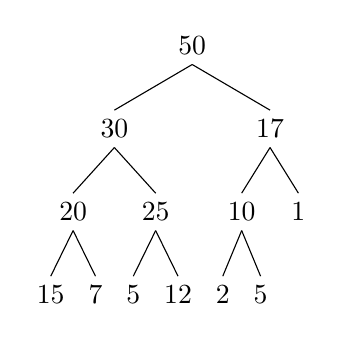
\begin{tikzpicture}
\Tree [.50 [.30 [.20 15 7 ] [.25 5 12 ] ] [.17 [.10 2 5 ] 1 ] ];
\end{tikzpicture}
&&
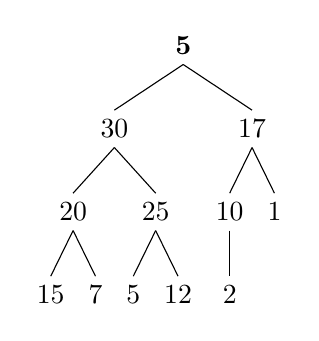
\begin{tikzpicture}
\Tree [.\textbf{5} [.30 [.20 15 7 ] [.25 5 12 ] ] [.17 [.10 2 ] 1 ] ];
\end{tikzpicture}
\\
\textbf{C}&&\textbf{D}&\\
&
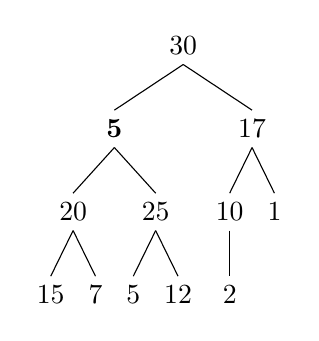
\begin{tikzpicture}
\Tree [.30 [.\textbf{5} [.20 15 7 ] [.25 5 12 ] ] [.17 [.10 2 ] 1 ] ];
\end{tikzpicture}
&&
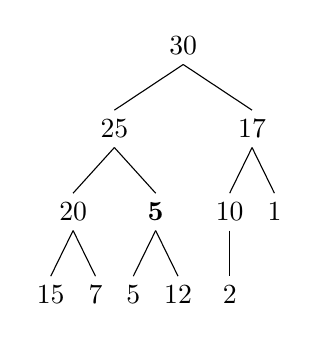
\begin{tikzpicture}
\Tree [.30 [.25 [.20 15 7 ] [.\textbf{5} 5 12 ] ] [.17 [.10 2 ] 1 ] ];
\end{tikzpicture}
\\
\textbf{E}&&&\\
&
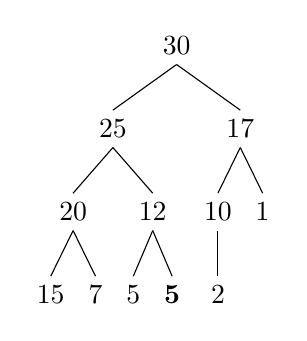
\begin{tikzpicture}
\Tree [.30 [.25 [.20 15 7 ] [.12 5 \textbf{5} ] ] [.17 [.10 2 ] 1 ] ];
\end{tikzpicture}
&&
\end{array}
$
\end{center}
\caption{\textbf{A} shows the tree before the root node is deleted; in \textbf{B} the node is removed and replace with the five from the lowest layer and in \textbf{C} to \textbf{E} this five sinks back downwards to its correct position.\label{fig:removing}}
\end{figure}



\end{document}
